\documentclass[article,12pt,onesidea,4paper,english,brazil]{abntex2}

\usepackage{lmodern, indentfirst, nomencl, color, graphicx, microtype, lipsum}			
\usepackage[T1]{fontenc}		
\usepackage[utf8]{inputenc}		

\setlrmarginsandblock{2cm}{2cm}{*}
\setulmarginsandblock{2cm}{2cm}{*}
\checkandfixthelayout

\setlength{\parindent}{1.3cm}
\setlength{\parskip}{0.2cm}

\SingleSpacing

\begin{document}
	
	\selectlanguage{brazil}
	
	\frenchspacing 
	
	\begin{center}
		\LARGE DESENVOLVIMENTO DE SISTEMA DE AVALIAÇÃO DA CONDIÇÃO FÍSICA DE ESTUDANTES DO ENSINO BÁSICO, TÉCNICO E TECNOLÓGICO.\footnote{Pesquisa realizada na área de Ciências da Saúde, financiada pela Fundação Rondônia de Amparo ao Desenvolvimento das Ações Científicas e Tecnológicas e à Pesquisa do Estado de Rondônia (FAPERO) e pelo Conselho Nacional de Desenvolvimento Científico e Tecnológico (CNPq).}
		
		\normalsize
		Miguel Amadio de Oliveira\footnote{Informações do Autor 1.Bolsista, miguel.amadio2@gmail.com, Campus Porto Velho Calama.} 
	Iranira Geminiano de Melo\footnote{Orientadora, iranira.melo@gmail.com, Campus Porto Velho Calama} 
	George Madson Dias Santos\footnote{Co-orientador, george.santos@ifro.edu.br, Campus Porto Velho Calama}  
	\end{center}
	
	% resumo em português
	\begin{resumoumacoluna}
		Na pesquisa tivemos por objetivo informatizar um questionário para o estudo da condição física dos alunos do Instituto Federal de Rondônia, do Campus Porto Velho Calama. Para atender a esse objetivo foram utilizadas as linguagens de programação CSS, Java Script, HTML e SQL. Tivemos como resultado uma ferramenta de coleta de dados capaz de interagir com o pesquisado, podendo ser utilizada também como instrumento educativo.
		
		\vspace{\onelineskip}
		
		\noindent
		\textbf{Palavras-chave}:Condicionamento Físico. Qualidade de Vida. Tecnologia.
	\end{resumoumacoluna}
	
	\section*{Introdução}
	
Condição física é o grau de desenvolvimento das capacidades físicas (TEIXEIRA, 1995), estando, portanto, relacionada com condicionamento físico que é uma capacidade alcançada pelo indivíduo afastado do sedentarismo. Também pode ser entendido como a resistência que o atleta ou o praticante de exercícios possui, como por exemplo, o tônus muscular, a capacidade de realizar contrações isométricas e isotônicas sem perda do tônus, sem dores e sem fadigas, como também denota a capacidade de realizar exercícios aeróbicos (corrida, pedalada) e anaeróbicos (levantamento de pesos) alternados (NAHAS, 2013).
Foi considerando a relação positiva entre a condição física e a saúde que tivemos como principal objetivo desenvolver um sistema avaliativo da condição física para ser utilizado em pesquisa e como ferramenta educativa pelos professores de Educação Física do ensino básico, técnico e tecnológico do Instituto Federal de Educação, Ciência e Tecnologia de Rondônia (IFRO), Campus Porto Velho Calama. Esse sistema é uma aplicação web capaz de hospedar ferramentas avaliativas utilizadas no estudo da atividade física, saúde e qualidade de vida.
	
	\section*{Material e Método}
	
	Na pesquisa foi desenvolvida uma aplicação web capaz de hospedar ferramentas avaliativas, no caso em questão foi codificado o questionário de “Avaliação da condição física”, descrito por Teixeira (1995). Como vantagem da utilização da aplicação em estudo situamos que ela possibilita um feedback automático ao participante da pesquisa com o resultado da avaliação individual, além de ter os dados armazenados automaticamente no banco de dados para posterior compilação e análise pelo grupo de pesquisadores.
	Para que pudéssemos desenvolver o sistema foram utilizadas as linguagens PHP, CSS, Java Script, HTML e SQL. Assim, o questionário, composto de dez questões, todas com alternativas de sim ou não, que foram dispostas em colunas, sendo a coluna da esquerda sim e a da direita não. A distribuição da pontuação ocorre da seguinte forma: a coluna da esquerda tem valor 0 e a da direita valor 1. A soma total da pontuação permite que classifiquemos os usuários em três categorias: (1 a 5 pontos) “Condição física insuficiente”, sendo fornecida também a mensagem “Você não está em boas condições físicas. Por isso, precisa praticar mais atividades físicas”; (6 a 7 pontos) “Condição física normal”; (8 a 10 pontos) “Boa condição física”.
	Na próxima fase do projeto a pesquisa será feita com os alunos do Instituto Federal de Rondônia do Campus Porto Velho Calama, e, temos a intenção de incluir na pesquisa todos os alunos do curso técnico integrado dos turnos matutino e vespertino.
	
	\section*{Resultados e Discussão}
	
	O resultado alcançado foi o desenvolvimento de um site onde está hospedado o questionário, conforme a figura 1. Após responder ao questionário o aluno deverá clicar em continuar e, então visualizar o resultado da condição física dele. Destacamos, uma vez mais, que o participante da pesquisa deve escolher entre duas alternativas para responder ao questionário: sim ou não (figura 1).
	
	\begin{figure}[h]
		\centering
		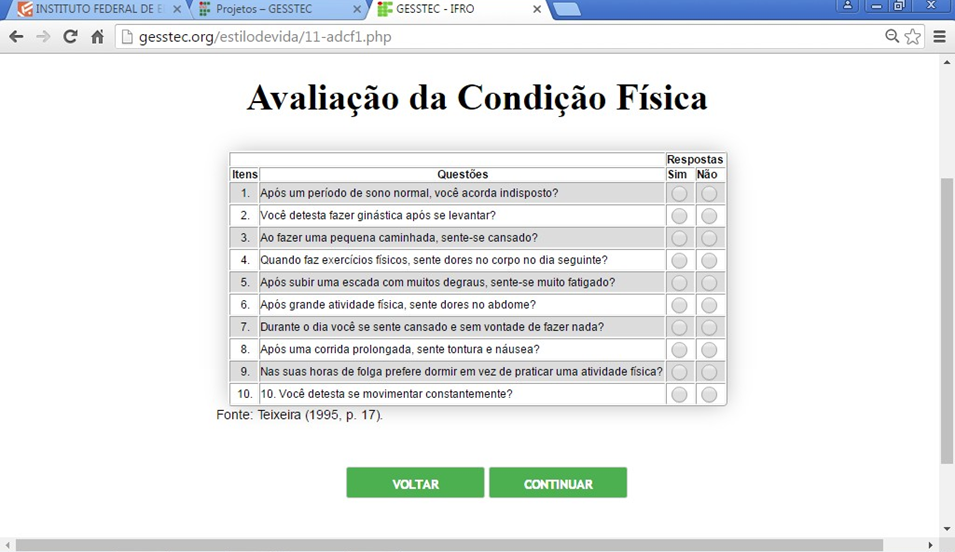
\includegraphics[width=0.4\linewidth]{pip13-1.png}
		\caption{Questionário Avaliação da Condição Física, Porto Velho, 2016.}
	\end{figure}
	
	A figura 2 representa um resultado do questionário lembrando que o respondente poderá ter a condição física dele classificada em “condição física insuficiente”, “condição física normal” ou “boa condição física”. No caso mostrado é atingida a pontuação sete e exibido o resultado de “condição física normal” para o respondente.
	
	\begin{figure}[h]
		\centering
		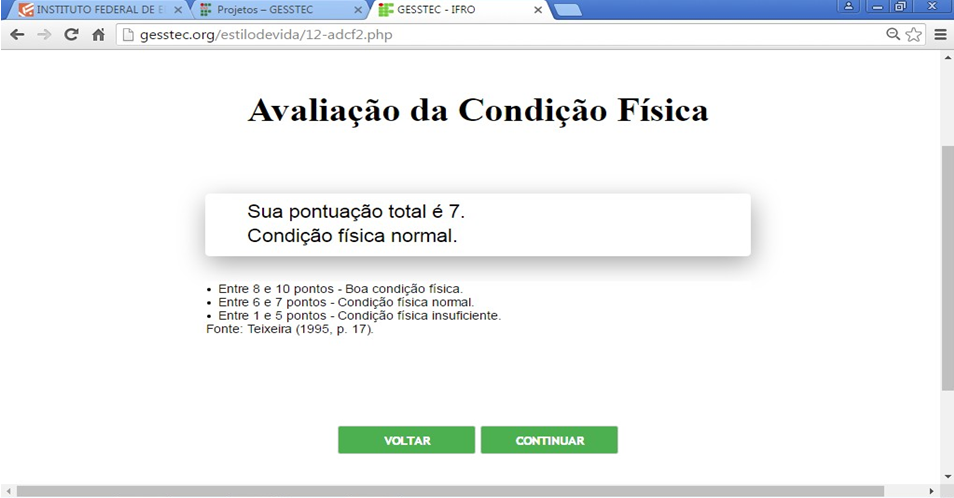
\includegraphics[width=0.4\linewidth]{pip13-2.png}
		\caption{Ilustração de feedack do questionário informatizado, Porto Velho, 2016.}
	\end{figure}

A partir do conhecimento da condição física o respondente pode aderir a um programa de condicionamento físico e melhorá-la. Para isso, Reis (2009) recomenda que esse programa deva seguir uma frequência de 3 a 5 vezes por semana, ser intercalados com dias de descanso, ter duração mínima de 15 minutos e ser desenvolvido em uma frequência cardíaca máxima de 60\% a 85\% ou conforme a condição física do indivíduo. O autor esclarece que em três meses consecutivos, essa programação conduz a resultados satisfatórios para a obtenção de um bom condicionamento físico.
	
	\section*{Conclusões}
	
	Conclui-se que a ferramenta desenvolvida possibilita aos alunos uma avaliação da condição física dele e, a partir desse conhecimento, a pessoa pode promover mudanças para que alcancem melhoria e consiga um melhor resultado em uma reavaliação, que poderá ser feita a qualquer momento. O armazenamento dos dados permite o estudo e acompanhamento da condição física dos alunos, contribuindo para que a coleta e análise de dados sejam dinâmicas e eficientes.
	
	\section*{Agradecimentos}
	À Pró-Reitor de Pesquisa, Inovação e Pós-Graduação (PROPESP/IFRO) e ao Departamento de Pesquisa, Inovação e Pós-Graduação (DEPESP/Campus Porto Velho Calama) pela oportunidade de divulgação da pesquisa e apoio ao Grupo de Estudos Saúde, Sociedade e Tecnologia (GESSTEC/IFRO).
	
	\section*{Instituição de Fomento}
	
	Fundação Rondônia de Amparo ao Desenvolvimento das Ações Científicas e Tecnológicas e à Pesquisa do Estado de Rondônia (FAPERO) e pelo Conselho Nacional de Desenvolvimento Científico e Tecnológico (CNPq).
	
	\section*{Referências}
	
\noindent NAHAS, Markus V. \textbf{Atividade Física, Saúde e Qualidade de Vida.} 6 ed. Londrina: Midiograf, 2013.

\noindent REIS, Jorge Luiz dos. \textbf{Representações sociais de profissionais da saúde a respeito de condicionamento físico.} Dissertação (mestrado), Universidade Estácio de Sá, Rio de Janeiro, 2009. Disponível em:<http://livros01.livrosgratis.com.br/cp116698.pdf>. Acesso em: 29, de abril de 2016.

\noindent TEIXEIRA, Hudson Ventura. \textbf{Educação Física e Desportos}: técnicas, táticas, regras e penalidades. São Paulo: Saraiva, 1995.
	
\end{document}